\documentclass{article}
\usepackage[utf8]{inputenc}
\usepackage[document]{ragged2e}
\usepackage{graphicx}
\usepackage[a4paper, total={6in, 8in}]{geometry}

\begin{document}
\begin{center}
       
    \Huge
    \textbf{SPECIFICATON} \\
     \huge
     \vspace{2.5cm}

     \vspace{0.5cm}
    Andreas Siggelkow\\
    Circuit Design \\
    \vspace{2.5cm}
    \large
    Swarnim Man Dangol(32283)\\
    Anand Chaudhary (32232)    \\
    \vspace{0.5cm}
  
    
\end{center}
\newpage
\tableofcontents


\newpage
  \begin{center}
    \section{History}

         \begin{tabular}{c|c }
         \hline
        DATE   & UPDATES \\
         \hline
        08.11.2020 & Document started \\
         \hline
        09.11.2020 & Document updated with Block diagram and Description \\
        
         \hline
       16.01.2021 & redid requirements and new block diagram\\
        \hline
        17.01.2021 & uploaded block diagrams and requried FSM's\\
        \hline
        18.01.2021 & Description of OSI-Layers \\
        \hline
         
\end{tabular}
\end{center}
\newpage
\section{Overview}

    The ASIC FPGA should be able to count the number of people entering a certain place with the help of three light curtains near the door, Also there is only doorway to come and exit. There are LED's that signal if the room can be entered,\textbf{Green} LED being \textbf{GO} (The room has not reached maximum capacity) and ,\textbf{Red} LED being \textbf{STOP} (The room has reached maximum capacity). The LED's are also accompanied by acoustic sounds that indicate if the room is full or if a person  has entered the room.
\vspace{2.5 cm}

\begin{center}

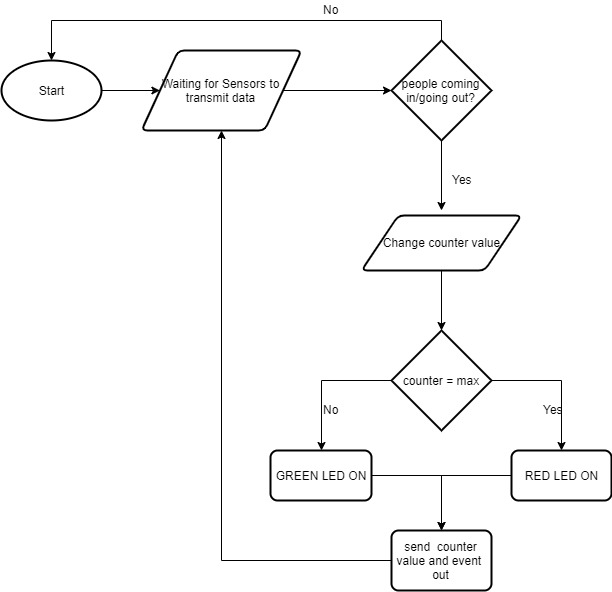
\includegraphics[width=12.5cm]{Untitled Diagram (2).jpg}\\
\vspace{0.5cm}
Fig 2 Flow-chart of design
\end{center}

\newpage
\section{ Requirements}
\subsection{General}
\begin{center}
	\begin{tabular}{|p{1.5cm}|p{3.5cm}|p{1.5cm}|p{2cm}|p{5.5cm}|}
		\hline
		\textbf{ID} & \textbf{Requirement} & \textbf{Priority} & \textbf{Verifiable} & \textbf{Description} \\
		\hline
		\hline
		1 &  \#persons &  High &  Testbench & The number of persons in a room must be known. \\
		\hline
		2 & max & High &  Testbench & The number of persons in a room must not exceed a given limit. \\
		\hline
		3 &  only one pers. & High & N/A & Only one person can either enter or leave the room at a time. \\
		\hline
		4 &  three light sensors & Medium & Testbench & Along the doorway, there are three light-curtains to allow directiontracking of possible visitors. \\
		\hline
		5 &  only one door & High & N/A & Only one door exists. \\
		\hline
	
		1 &  RED-LED &  High & Testbench & The maximal number of persons reached. \\
		\hline
		2 & GREEN-LED & High & Testbench & The maximal number of persons not reached. \\
		\hline
	
	
		1 &  Entered-Sound & High & N/A & A person entered the room, play a unique sound. \\
		\hline
		2 & Left-Sound & High & N/A & A person left the room, play a unique sound. \\
		\hline
		3 &  Stop-Sound & High & N/A & The room is full, play a unique sound. \\
		\hline
	\end{tabular}
\end{center}

\subsection{UART}
\begin{center}
    
\begin{tabular}{|p{1.5cm}|p{3.5cm}|p{1.5cm}|p{2cm}|p{5.5cm}|}
		\hline
		\textbf{ID} & \textbf{Requirement} & \textbf{Priority} & \textbf{Verifiable} & \textbf{Description} \\
		\hline
	
		\hline
		1 & 9600 baud & High &  Testbench & The speed of the serial transmission should be set to 9600 baud. \\
		\hline
		2 &  8 bit & High & Testbench & The data width of the serial transmission should be set to 8 bit. \\
		\hline
		3 &  no parity & High & Testbench & The serial transmission should not be checked with a parity bit. \\
		\hline
		4 &  one stop bit & High  & Testbench & The serial transmission should have only one stop bit. \\
		\hline
		6 &  \#persons & High &  Testbench &  The \#persons should be transmitted to a PC. \\
		\hline
		\end{tabular}
		\end{center}
		\newpage
		\subsection{PC and S3Interface}
		\begin{center}
	
		\begin{tabular}{|p{1.5cm}|p{3.5cm}|p{1.5cm}|p{2cm}|p{5.5cm}|}
			\hline
	
		\hline	
		1 & PC: language & Medium & N/A &  Information should be displayed on a PC, the language is C++. \\
		\hline
		2 & PC: timestamp & Low & N/A  & Every event should have a unique timestamp. \\
		\hline
	
		\hline
		1 & S3: interface & Low & Testbench & Use a three wire IF. \\
		\hline
		2 & S3: events & Low & Testbench & All events should be transmitted via the three wire IF. \\
		\hline
		3 & S3: \#persons & Low  & Testbench & The \#persons should be transmitted via the three wire IF. \\
		\hline
		\end{tabular}
		\end{center}
\newpage
\section{Architectural Concepts}
    
    
    \vspace{1.5 cm}

\subsection{Synchronous circuit}

The blocks designed are all synchronized with the clock so the changes occur only when there is a rising edge of the clock.

\vspace{1.5 cm}

\subsection{Reset}
In this design the blocks uses an active low reset signal as the built in reset buttons on the MAX10 boards are active low signals.

\vspace{1.5 cm}

\subsection{Three Process Architecture}
The VHDL design, especially FSM's are built with three different processes(state transition, clock trigger, outputs) for easy readability of the code and for the simplification of the code.
\vspace{1.5 cm}
\subsection{Moore FSM}
The VHDL design specifically uses a Moore FSM structure in every FSM present in the design, as the outputs are only affected by the change in states, It simplifies the code required to construct a FSM.
\newpage


\newpage

\begin{center}
\section{Top-level diagram}
\vspace{1 cm}
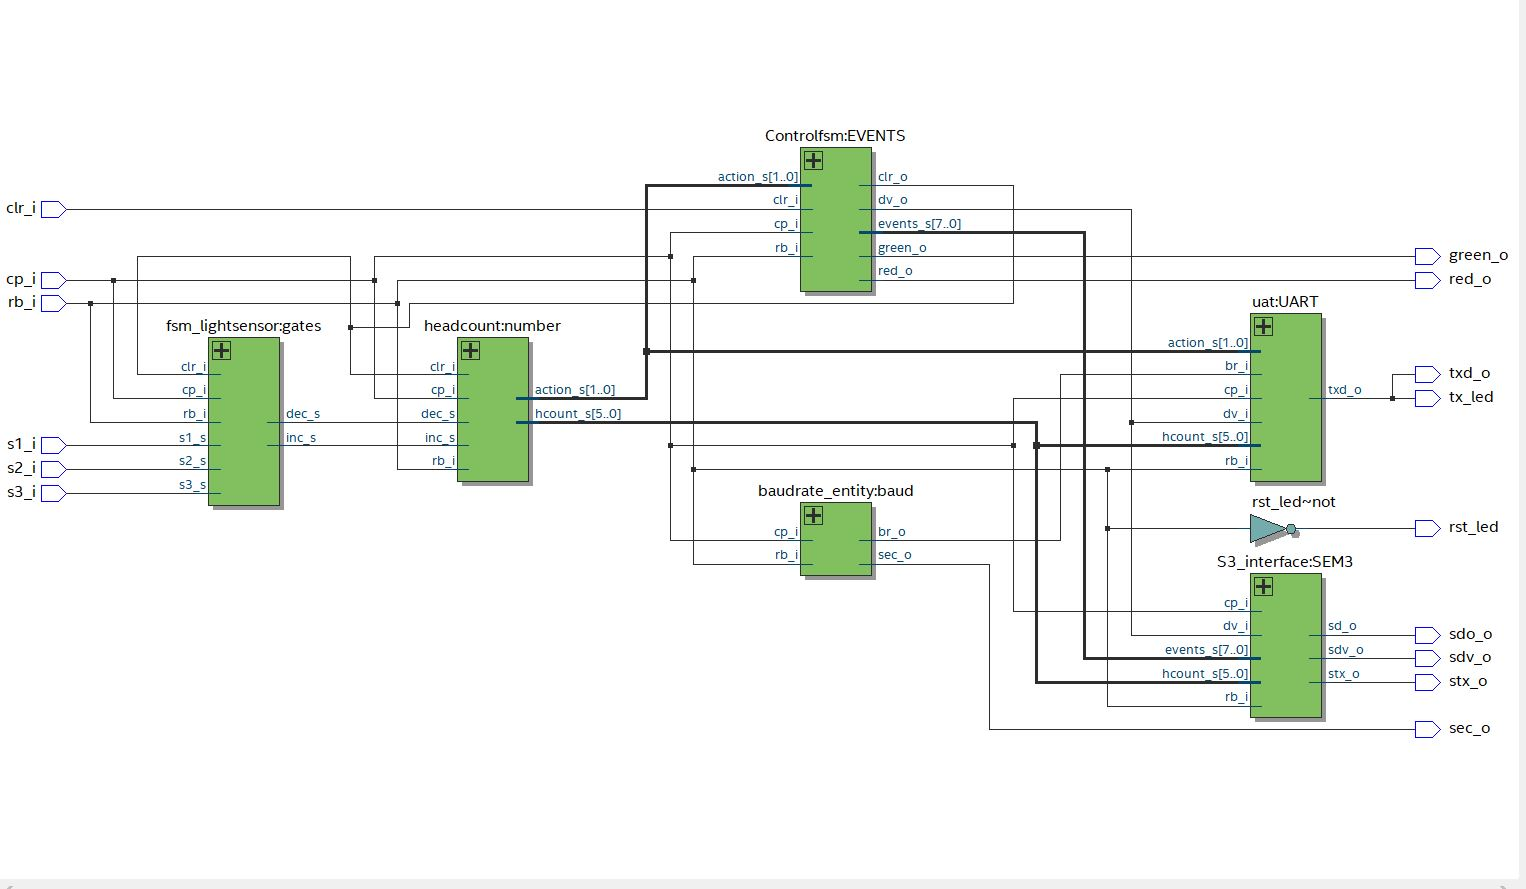
\includegraphics[width=17cm]{top.JPG}
\end{center}
\newpage
\begin{center}
\subsection{Input and Output Signals}
    
\end{center}

    \begin{center}
             \begin{tabular}{|c|c|c|c|}
\hline
         
        Signal& Full name & Type& Description \\
        \hline
        \hline
        cp\_i& System Clock & I&  System clock of 10 MHz \\ 
        \hline
        rb\_i & Reset & I& reset, active low \\
        \hline 
        s1\_i & first sensor & I &signal from first sensor \\
        \hline
        s2\_i & Second sensor & I& signal from second sensor\\
        \hline 
        s3\_i & thrid sensor & I & signal from third sensor\\
        \hline
        clr\_i & Clear counter & I &clear and restart headcount \\
        \hline 
        red\_o & Red LED & O &enables red LED \\
        \hline
        grn\_o  & Green LED & O & enables green LED \\
        \hline
      
        txd\_o & Serial data out & O & serial data out to the PC through RS232\\
        \hline
        sdo\_o  & serial data output & O & drives S3 or µC\\
        \hline 
        sdv\_o & serial data valid & O &drives S3 or µC\\
        \hline
        stx\_o & serial data transfer active & O & drives S3 or µC \\
        \hline 
        tled\_o & txd-LED & O & LED on when serial data is being transferred\\
        \hline
        
           \end{tabular}
    \end{center}  
    \vspace {1.5cm}
\center{\subsection{Internal Signals}}

    \begin{center}
         \begin{tabular}{|c|c|c|c|}
         \hline
        Signal& Full name & Type& Description \\
        \hline
        \hline
       
        \hline 
        br\_s&  Baudrate signal & S &  Baudrate \\
        \hline
        inc\_s & increment counter & S & high when a person walks in\\
        \hline
        dec\_s& decrements counter & S & high when a person goes out \\
        \hline
        clr\_i & Clear counter & S & clear and restart headcount \\
        \hline 
         hcount\_s & Headcount & S & number of people  \\
        \hline
        event\_s & Event (6-bit) & S&  status signal !,+,- \\
        \hline 
        action\_s  & action(2-bit) & S& signals people coming in, going out or max number is reached\\
        \hline
        dv\_s  & Data valid & S& Signals UART and S3inteface to start\\
        \hline
        
           \end{tabular}
    \end{center}  
    
    \newpage

    

\newpage

\section{Baud-rate Generator}
This block handle the dividing of the 12 MHz System-Clock to 9600 baud (br\_s)for the Serial-Transmission between the UART and the PC. It also handles a pulse signal(sec\_o), which is sent  every second by dividing the clock with an appropriate pre-scaler value.
\begin{center}

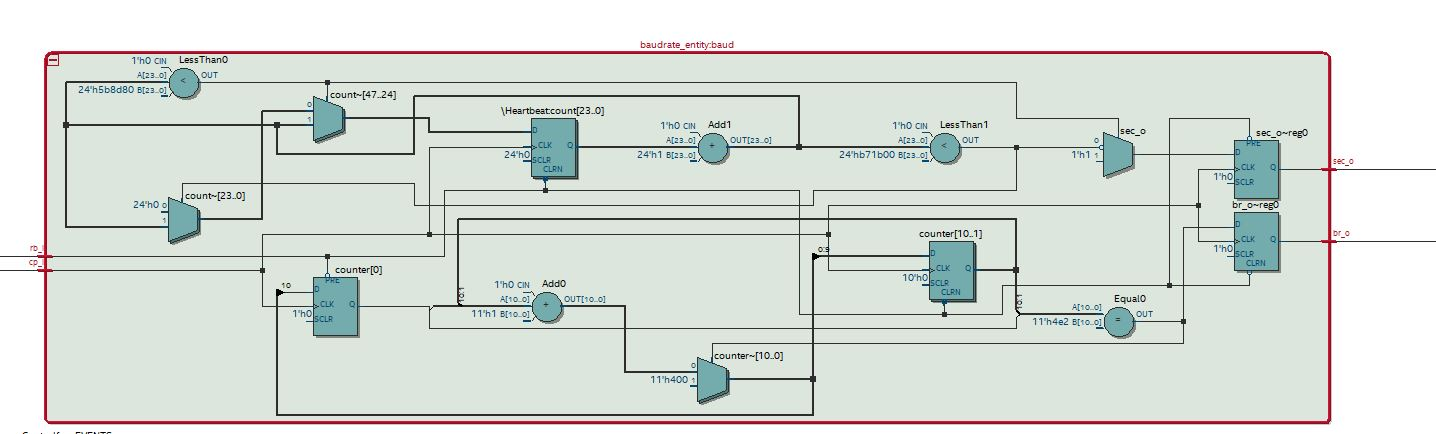
\includegraphics[width=15cm]{baudrate.JPG}
    Fig 6. Shows the block of the Baud-rate Block.

\end{center}
    \vspace{2cm}
  \begin{center}
        
          \begin{tabular}{|c|c|c|c|}
         \hline 
        Signal & Full name & Type &Description \\
        \hline
        \hline
        cp\_i & System Clock & I &System clock of 12 MHz \\ 
        \hline
        rb\_i & Reset & I & reset, active low \\
        \hline 
        br\_s & Baudrate signal & O & Baudrate \\
        \hline
        sec\_o & Heartbeat signal & O & pulse signal after every second\\
        \hline
          \end{tabular}
       
     
\end{center}
 Table 6. (I/O) Baud-rate Block
  
  \vspace{2.5cm}
 
  \newpage
\section{Light-sensor}
The light sensor block takes the input from the light-sensors and sends an output signal to the headcount block. For people coming in,it sends an increment signal (inc\_s) and for people going out it sends a decrement signal(dec\_s).For this, the first sensor is s1\_i and the  third sensor is s3\_i.

\begin{center}

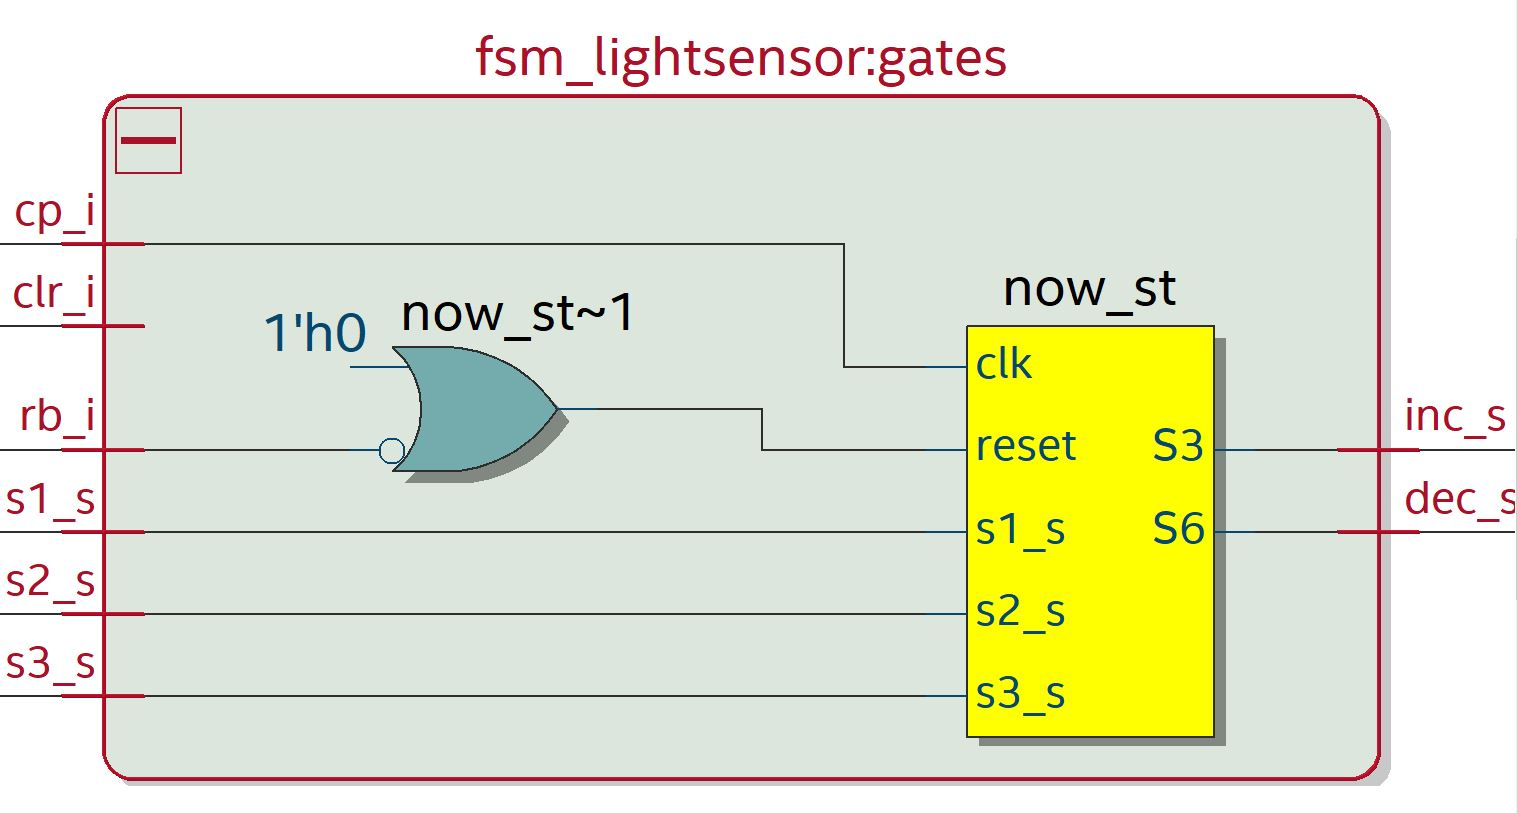
\includegraphics[width=10cm]{ls.JPG}
\end{center}
    Fig 7. lightsensor block
    \vspace{2cm}
 \begin{center}
           \begin{tabular}{|c|c|c|c|}
         \hline
        Signal   & Full name  & Type & Description\\
        \hline
        \hline
        cp\_i  & System Clock  & I & System clock of 12 MHz \\ 
        \hline
        rb\_i  & Reset   & I & reset, active low \\
        \hline 
        s1\_i &   first sensor  & I & signal form first sensor \\
        \hline
        s2\_i &   second sensor & I & signal form second sensor\\
        \hline
        s3\_i &   third sensor & I & signal form third sensor \\
        \hline
        inc\_s &  increment counter & O & high when peole walks in \\
        \hline
        dec\_s &  decrement counter  & O & high when people goes out \\
        \hline
          \end{tabular}
          \vspace{0.5cm}
          
          Table 7.(I/O) Lightsensor block
       \end{center}
       \newpage
       \subsection{LS FSM}
       \begin{center}
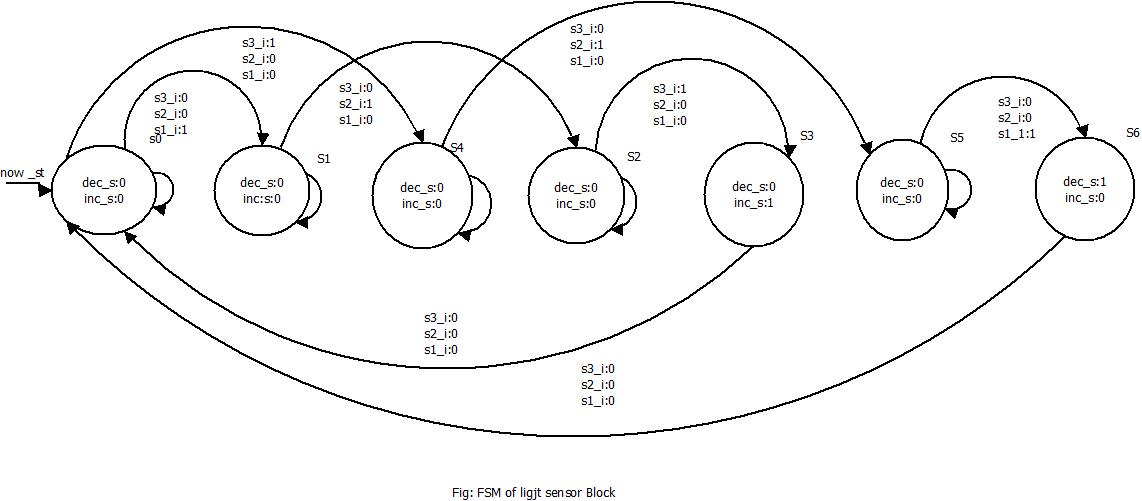
\includegraphics[width=15cm]{lightsensorfsm.jpeg}
Fig 7.1 FSM of Ligtsensor block
\end{center}


\vspace{2cm}
 \begin{center}
  \begin{tabular}{|c|c|c|c|}
         \hline
        State& Next State& Condition(s3\_i.s2\_i.s1\_i)   & Outputs(dec\_s.inc\_s)\\
        \hline
        \hline
        S0(initial state) & S1 & 001 & 00 \\ 
        \hline
         S0(initial state) & S4 & 100 & 00 \\ 
        \hline
        S1(person enters) & S2 & 010 & 00 \\
        \hline 
        S2(second sensor passed) & S3 & 100 & 00 \\
        \hline
        S3(Third sensor passed) & S0 & 000 & 01\\
        \hline
          S4(person leaves)& S5  & 010   & 00\\  
        \hline
        S5(second sensor passed)   & S6    & 001   & 00 \\
        \hline 
        S6(First sensor passed) & S0   & 000  & 10 \\
        \hline
       
          \end{tabular}
          \end{center} 7.1 State-transition table \\
       
          \vspace{1cm}
 
          
          \newpage
\section{Control}
This block takes in incoming signals passed from the light sensor block, according to that  sends the output  and an enable signal to the UART and the S3interface. The outputs are selected through a Finite-State-Machine(FSM) designed in the block.

\vspace{0.5cm}
\begin{center}

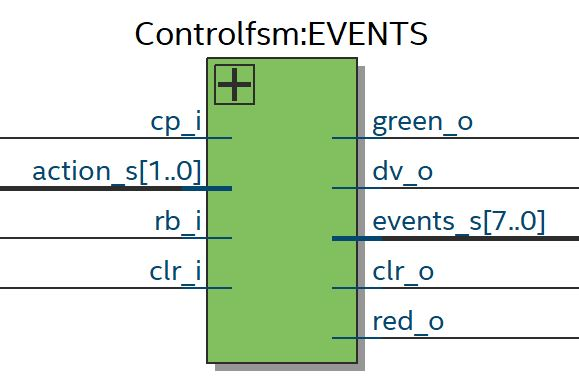
\includegraphics[width=7cm]{cntrol.JPG}
\end{center}
Fig 8. Controlfsm block

\vspace{0.5cm}
 \begin{center}
           \begin{tabular}{|c|c|c|c|}
         \hline
        Signal & Full name & Type & Description \\
        \hline
        \hline
        cp\_i & System Clock & I &System clock of 12 MHz \\ 
        \hline
        rb\_i & Reset & I & reset, active low \\
        \hline 
    
        green\_o & green out  & O &  Green led \\
        \hline
        red\_o & red out   & O & Red LED \\
        \hline
        action\_s &  action & I& signals people coming in, going out or max number is reached\\
        \hline
        event\_s &  event(6-bit) & O &  status signal !,+,- \\
        \hline
        dv\_s  &  Data valid  & O & Signals UART and S3inteface to start\\
        \hline
        clr\_i  &Clear in & I & Clears everything if high \\
        \hline
        clr\_o  & Clear out & O & Clears everything if high \\ 
        \hline
          \end{tabular}
       
\end{center}
   \vspace{0.25cm}
      Table 8. (I/O) of the Control-Block
\newpage

\subsection{Control FSM}
\begin{center}

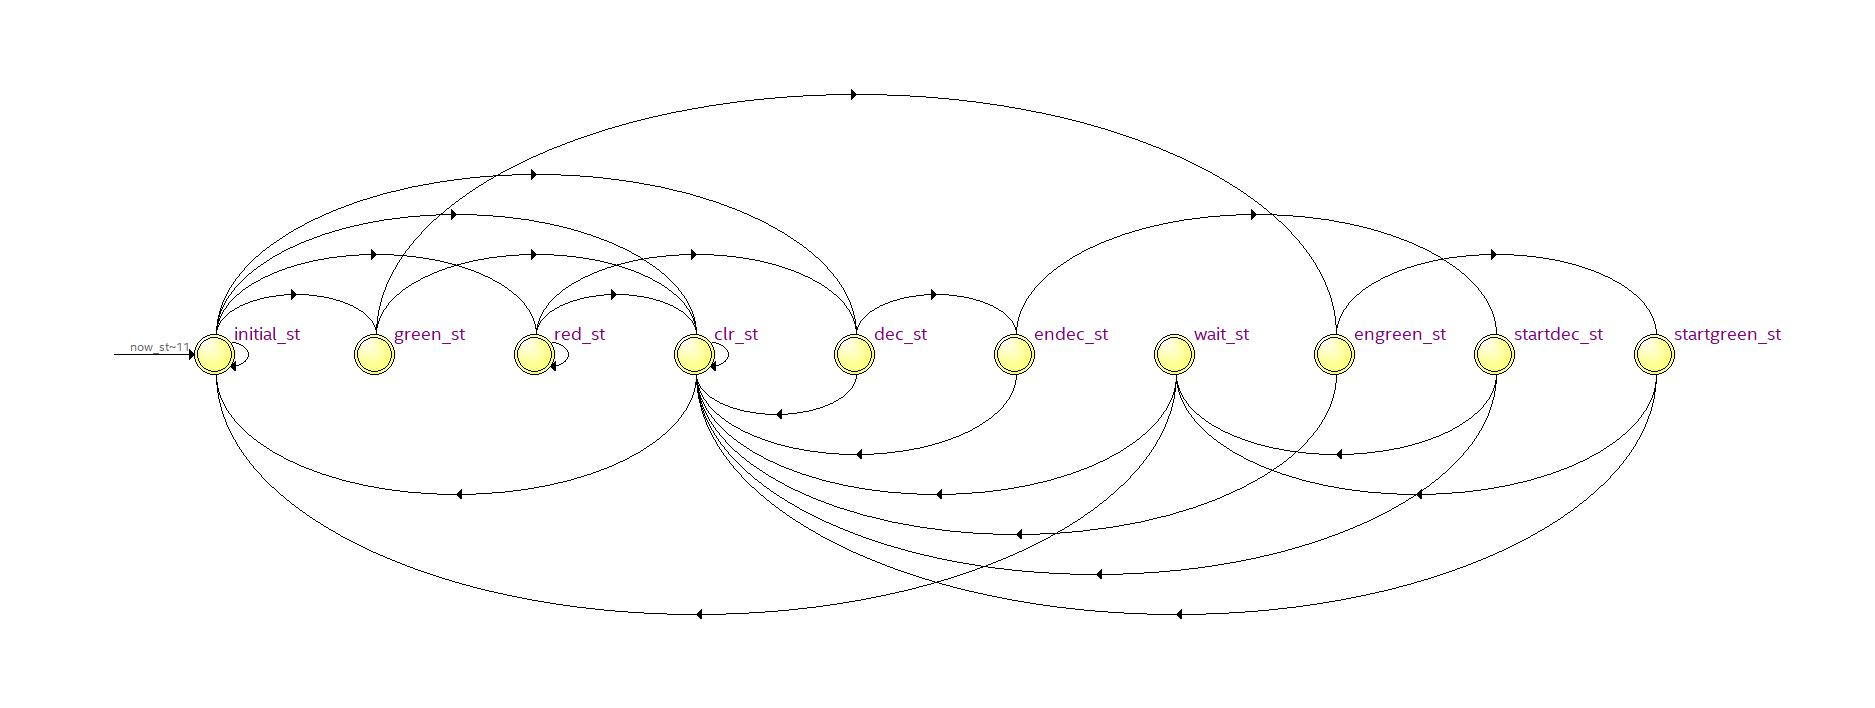
\includegraphics[width=15cm]{controlfsm.jpg}
\end{center}

    Figure 5.1 FSM Control
    
    \vspace{0.5cm}
  \begin{center}
         \begin{tabular}{|c|c|c|c|c|}
         
         \hline
         
        State & Next State & Condition & Outputs &events\_s\\
        &&(action\_s)& green\_s.red\_s.dv\_s.clr\_o &\\
        \hline
        \hline
        initial\_st& green\_st& 01 & 0000 &000000\\ 
        \hline
        initial\_st& red\_st&  11 & 000 & 000000\\ 
        \hline
        initial\_st& dec\_st& 10 &  0000 & 000000\\ 
        \hline
        green\_st & engreen\_st & 01 & 1000 & 00101011 \\
        \hline 
        dec\_st  &  endec\_st & 10 & 0000 & 00101101\\
        \hline
        red\_st &   red\_st & 11 & 0110 & 00101011\\
        \hline
        engreen\_st &   startgreen\_st& 01 & 1010 & 00101011 \\
        \hline
        endec\_st &   startdec\_st & 10 & 0010 &  00101101 \\
        \hline
        startgreen\_st &   wait\_st & 01 & 1000 & 00101011\\
        \hline
        startdec\_st &   wait\_st & 10 & 0000&   00101101\\
        \hline
        wait\_st &  initial\_st & 00 & 0000 &  00000000\\
        \hline
        clr\_st &   initial\_st & 00 & 0001 &  00000000\\
        \hline
          \end{tabular}
          \end{center}
          Table 8.1 State-transition
          \newpage
\section{Headcount}
This block with the given inputs( inc\_s  or dec\_s)  updates the number of people inside the room, by increasing and decreasing the number of people. further more it sends out an 2-bit signal to the Control block, which indicates the events taking place like people coming in, going out or the room is full or empty.

\begin{center}

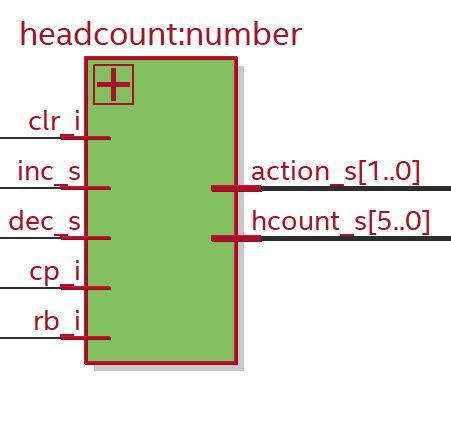
\includegraphics[width=5cm]{hdcnt.JPG}
\end{center}
Fig.9 Headcount block
\vspace{0.5cm}
 \begin{center}
           \begin{tabular}{|c|c|c|c|}
          \hline
        Signal & Full name & Description \\
        \hline
        \hline
        cp\_i & System Clock & I & System clock of 12 MHz \\ 
        \hline
        rb\_i & Reset & I &  reset, active low \\
        \hline 
        inc\_s &   increment counter & I &   high when peole walks in \\
        \hline
        dec\_s &   decrement counter & I &   high when people goes out \\
        \hline 
         action\_s  & action(2-bit) & O &   signals people coming in, going out or max number is reached\\
         \hline
           hcount\_s &   Headcount & O &   number of people  \\
           \hline
         
          \end{tabular}
\end{center}
Table.9 (I/O) of Headcount block


\newpage

\section{UART}
The UART block takes in  the inputs and then with the help of a fsm it loads the data to  8-bit register and transfer the given data out  to serially with the help of an multiplexer. This data is sent to the PC at 9600bps, 8bits without a parity-bit and with 1 stop-bit.

\begin{center}

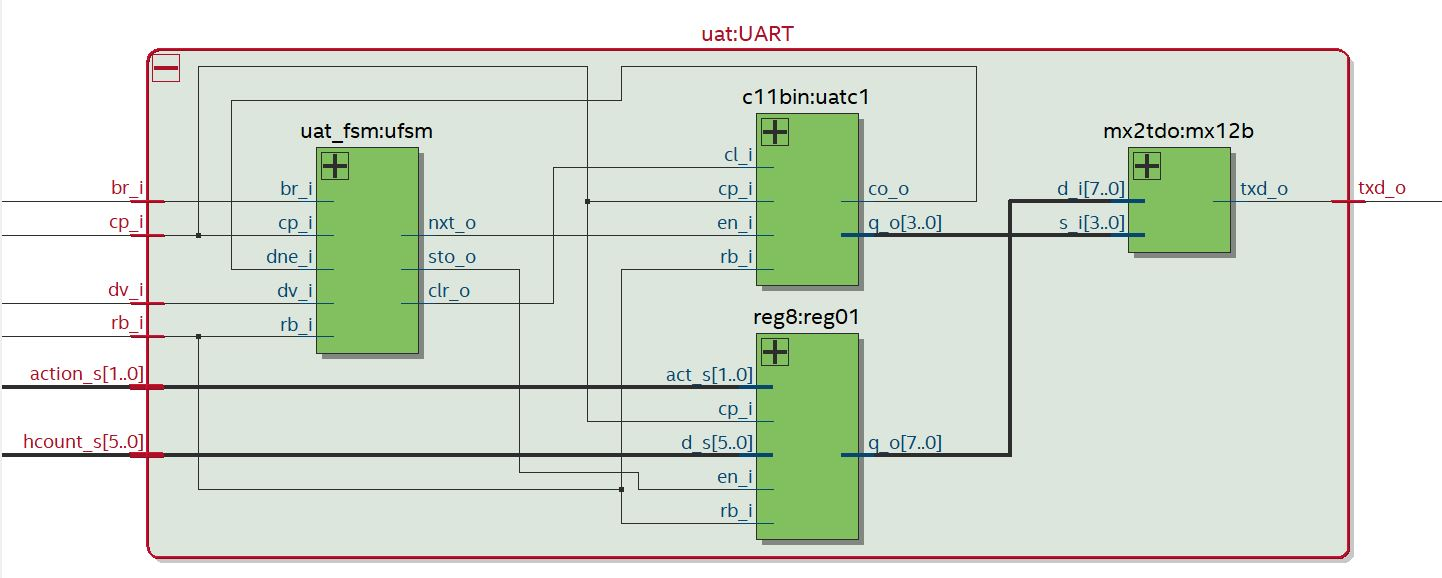
\includegraphics[width=15cm]{uart.JPG}
\end{center}
Fig 10. UART block
\vspace{0.5cm}
 \begin{center}
         \begin{tabular}{|c|c|c|c|}
         \hline
        Signal & Full name & Type & Description \\
        \hline
        \hline
        cp\_i & System Clock & I & System clock of 12 MHz \\ 
        \hline
        rb\_i &   Reset & I & reset, active low \\
        \hline 
        br\_i &   Baudrate signal & I & Baudrate \\
        \hline
       action\_s & action(2-bit) & I & signals people coming in, going out or max number is reached\\
        \hline 
         hcount\_s & Headcount & I &   number of people  \\
         \hline
         clr\_o & clear signal & S & clears the components inside the block \\
        \hline
        nxt\_o & next bit & S &  signals next bit to be transferred from the multiplexer \\
        \hline
        sto\_o & load register & S & fill the register \\
        \hline
         q\_o & 4-bit & S & counter out \\
        \hline
        c\_o & carry out & S &  carry high when last bit is reached \\
        \hline
         txd\_o &  Serial data out &  O & serial data out to the PC through RS232\\
        \hline
        
        \end{tabular}
\end{center}
Table 10. (I/O) of UART block
\vspace{0.5cm}


\begin{center}

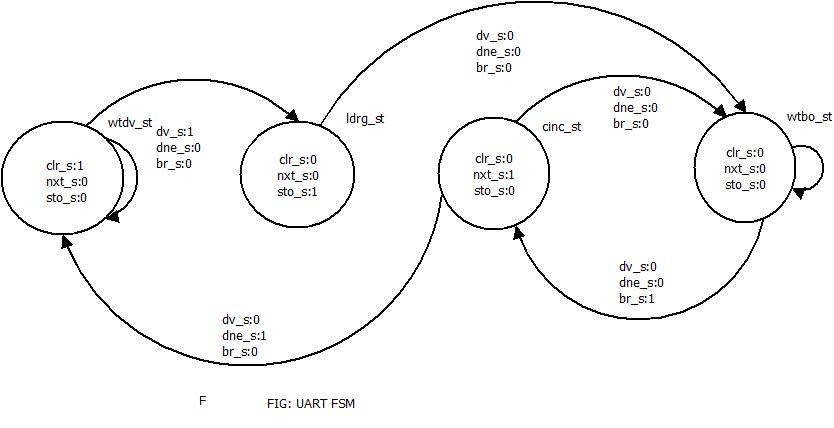
\includegraphics[width=17cm]{UART FSM.jpeg} 
\end{center}
\subsection{FSM}
Fig 10.1 UART FSM
\vspace{0.5cm}
  \begin{center}
  \begin{tabular}{|c|c|c|c|}
         \hline
          State & Next State & Condition & Outputs \\
        &&(dv\_s.dne\_s.br\_s)&(clr\_s.nxt\_s.sto\_s)\\
        \hline
        \hline
        wtdv\_st(wait for data valid) & ldrg\_st & 100 & 100\\ 
        \hline
        ldrg\_st(load register) & wtbo\_st & 000 & 001 \\
        \hline 
      
        cinc\_st(next bit) & wtdv\_st &  010  & 010  \\
        \hline
         cinc\_st(next bit) & wtbo\_st &     000   & 010  \\
        \hline
        wtbo\_st(wait for baud) & cinc\_st &   001 & 000\\
        \hline
          \end{tabular}
          \end{center}
          Table 10.1 state transition of UART FSM
          
\newpage
\subsection{Multiplexer}
The Multiplexer transfer data according to the input it gains from the 4-bit counter which only counts till 12 . So for "0000" it transfer's the first bit and soon till it reaches the end bit, after that it sends a stop signal(dne\_i) to stop the fsm. 
\begin{center}

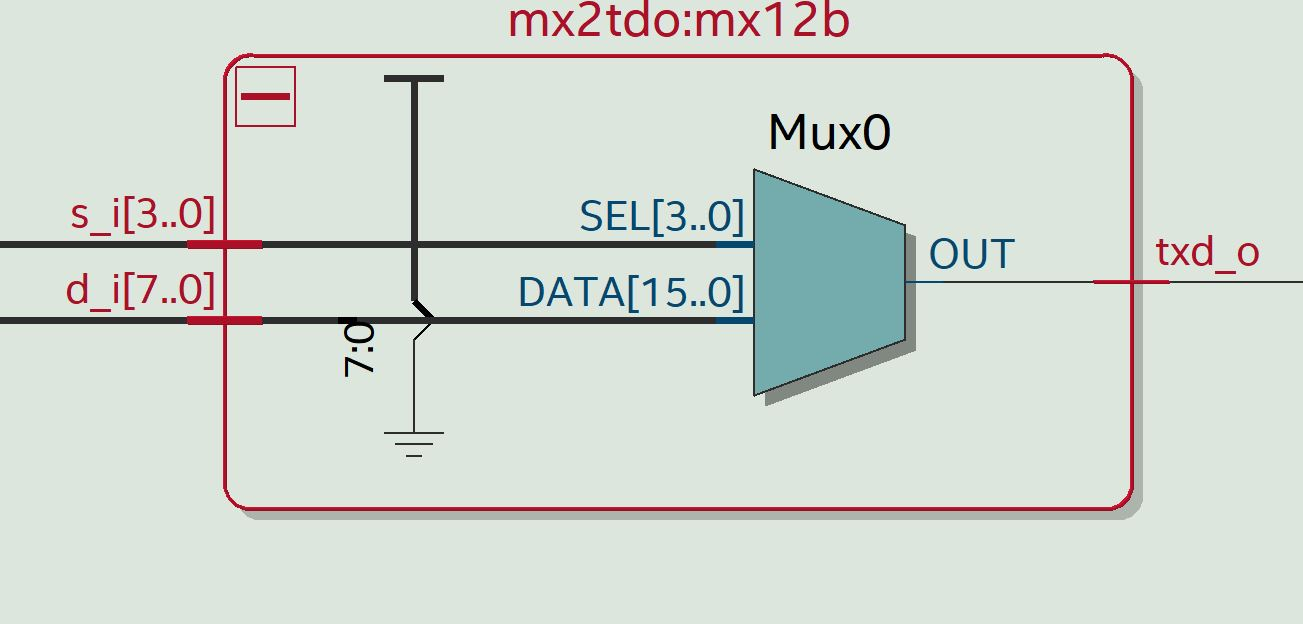
\includegraphics[width=12cm]{multiplexer.JPG}
.
\end{center}
Fig 10.2 multiplexer(UART MUX)
\vspace{1.5cm}
    \begin{center}
    \begin{tabular}{|c|c|c|c|}
        \hline 
        Signal  &  Full name & Type & Description \\
        \hline
        \hline
        s\_i &  4-bit selector & I &   Selector  \\ 
        \hline
        d\_i &  8-bit data & I &  Loaded data \\
        \hline 
        txd\_o &   1-bit out & O & Serial data out\\
        \hline 
        \end{tabular}
        \end{center}
        Table 10.2 UART-multiplexer
        

\newpage
\subsection{Register}

The register is an 8-bit register, storing the headcount(hcount\_s) and the action(action\_s). As soon as it receives the enable signal from the  UART.

\vspace{1cm}
\begin{center}

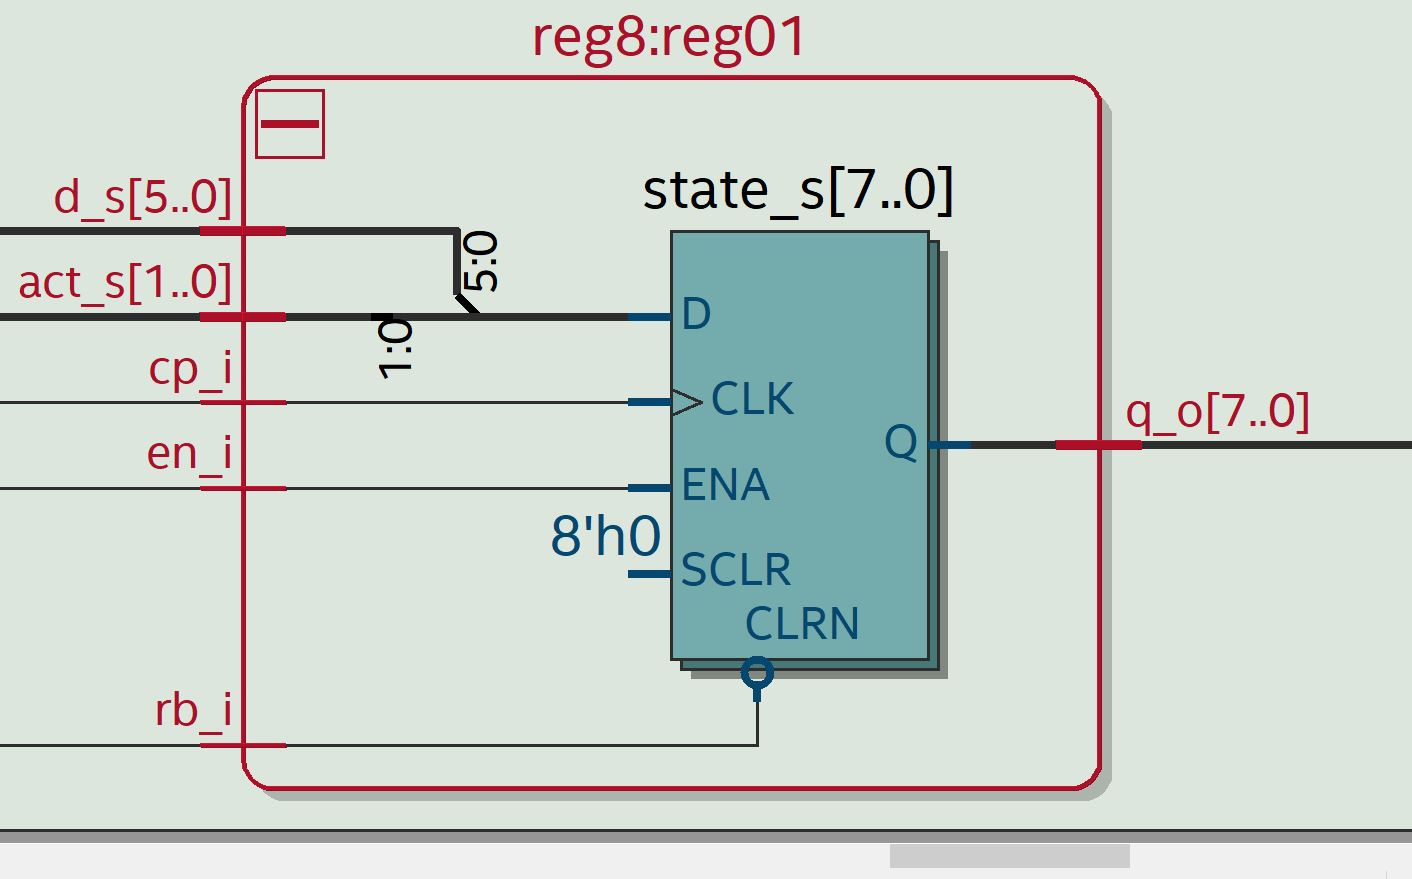
\includegraphics[width=10cm]{reguat.JPG}
\end{center}
Fig 10.3 UART-register

\vspace{1 cm}
\begin{center}
           \begin{tabular}{|c|c|c|c|}
        \hline 
        Signal  &  Full name & Type & Description \\
        \hline
        \hline
        cp\_i & clock & I & Sys clock of 12 MHz \\
        \hline
        rb\_i & reset & I & active low \\
        \hline
        en\_i & enable & I & start register  \\
        \hline
        d\_s & 6-bit data & I &number of people   \\ 
        \hline
        action\_s &  2-bit data  & I & +-! \\
        \hline 
        q\_o &   8-bit data & O & stored data\\
        \hline 
          \end{tabular}
\end{center}
Table 10.3 UART-register
\newpage
\section{S3 Interface}
This  block also like the UART takes in inputs from the Control block and with the help of a fsm loads the data to a 16-bit register  and transfers the given data out to a Micro-controller. It sends out three outputs,which indicates the data trasfer is begining(stx\_o), the data coming in is valid(stv\_o) and the data(sto\_o).


\begin{center}

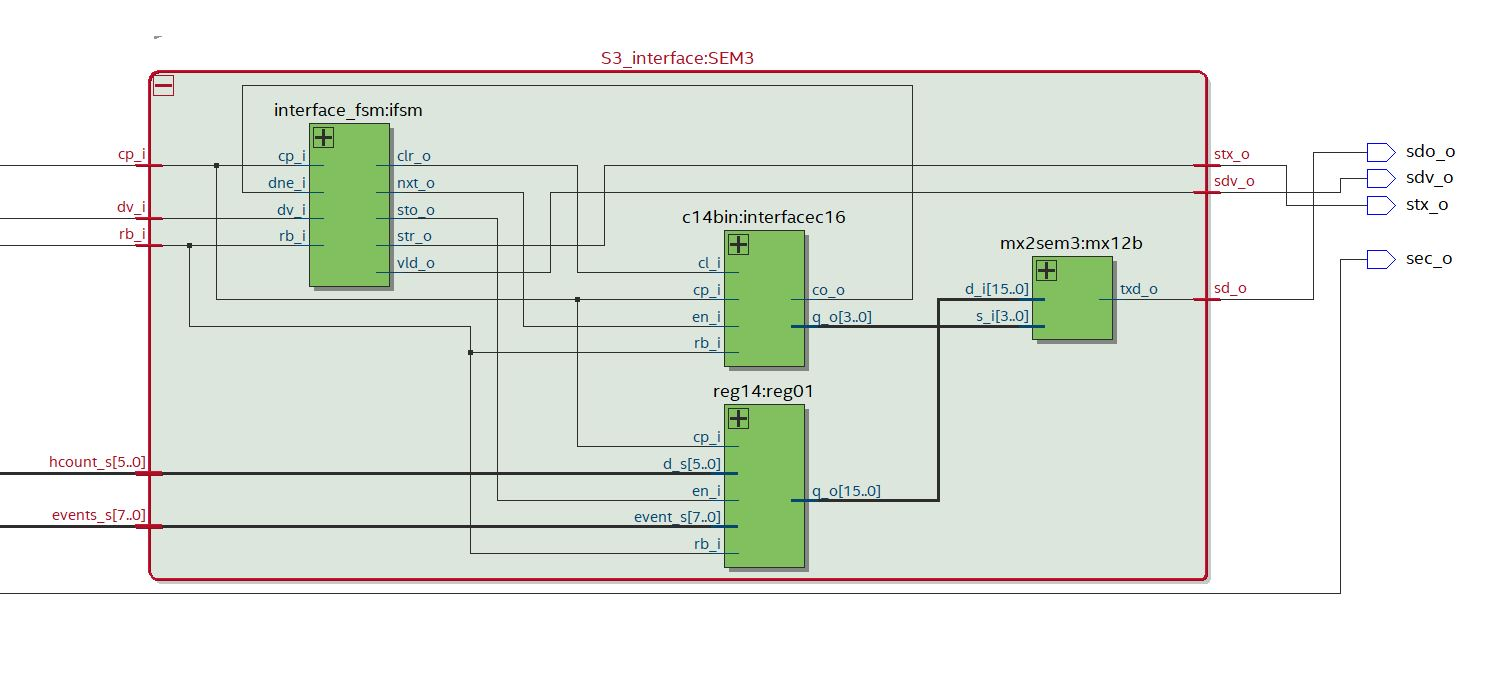
\includegraphics[width=15cm]{s3.JPG}
\end{center}
Fig 11. S3 Interface Block
 \begin{center}
           \begin{tabular}{|c|c|c|c|}
        \hline 
        Signal  &  Full name & Type & Description \\
        \hline
        \hline
        cp\_i & System Clock & I &   System clock of 12 MHz \\ 
        \hline
        rb\_i &   Reset &  I &reset, active low \\
        \hline 
        sdo\_o &   serial data output & O & drives S3 or µC\\
        \hline 
        sdv\_o &   serial data valid &  O &  drives S3 or µC\\
        \hline
        stx\_o &     serial data transfer active & O &   drives S3 or µC \\
        \hline
          hcount\_s     & Headcount & I &  number of people  \\
        \hline
        event\_s &   Event (6-bit) & I & status signal !,+,- \\
        \hline 
        dne\_s   & last bit reached & S & signals last bit is transferred\\
        \hline
        en\_i  & enable signal & S & starts the  respective component \\
        \hline
        clr\_o & clear signal & S & clears the components inside the block \\
        \hline
        vld\_o & valid data & S & signals the out going data is valid \\
        \hline
        nxt\_o & next bit & S &  signals next bit to be transferred from the multiplexer \\
        \hline
        str\_o & transfer start & S&  out going data transfer active \\
        \hline
        sto\_o & load register & S & fill the register \\
        \hline
        q\_s & 4-bit & S & counter out \\
        \hline
        c\_o & carry out &  S & carry high when last bit is reached \\
        \hline
          \end{tabular}
\end{center}
Table 11. (I/O) S3 Interface Block 
\vspace{1 cm}
\subsection{FSM}
\begin{center}

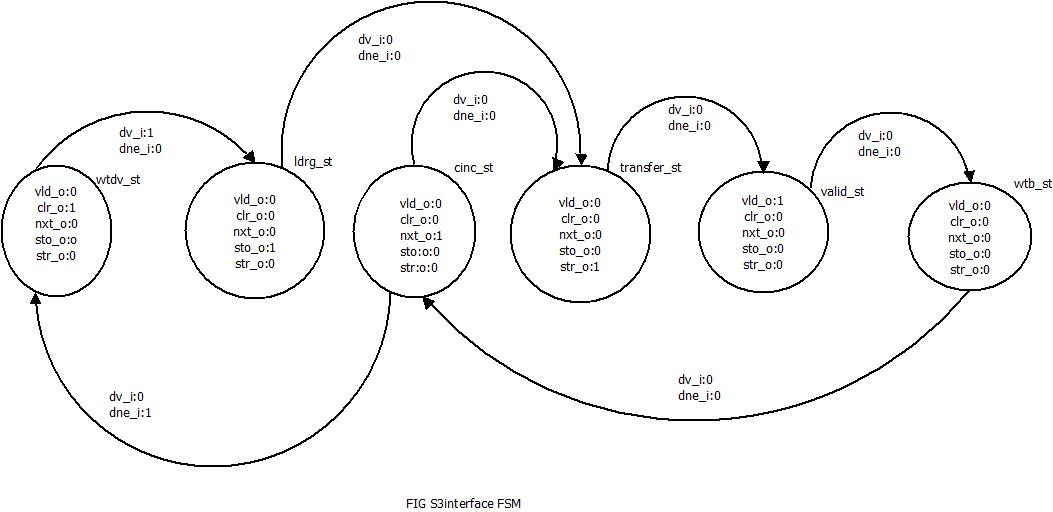
\includegraphics[width=15cm]{S3interface.jpeg}
\end{center}
Fig 11.1 S3interface FSM
\vspace{1 cm}
\begin{center}
  \begin{tabular}{|c|c|c|c|}
         \hline
          State & Next Stats & Condition & Outputs \\
        &&(dv\_i.dne\_i)&(vld\_o.clr\_o.nxt\_o.sto\_o.str\_o)\\
        \hline
        \hline
        wtdv\_st(wait for data valid) & ldrg\_st & 10 & 01000\\ 
        \hline
        ldrg\_st(load register & transfer\_st & 00 & 00010 \\
        \hline 
        cinc\_st(next bit & transfer\_st & 00 & 00100   \\
        \hline
        cinc\_st(next bit) & wtdv\_st & 01  & 00100   \\
        \hline
        transfer\_st(start transfer)   & valid\_st &  00 &00001\\
        \hline
        valid\_st(data valid)&  wtb\_st & 00 & 10000\\
        \hline
        wtb\_st(wait) & cinc\_st & 00 & 00000\\
         \hline
          \end{tabular}
          \end{center}
          Table 11.1 State-transition
\newpage
\subsection{Multiplexer}
16-bit-Mux for the S3interface. The data which needs to be sent are selected through a counter which counts to the required number of bits.

\vspace{1 cm}
\begin{center}

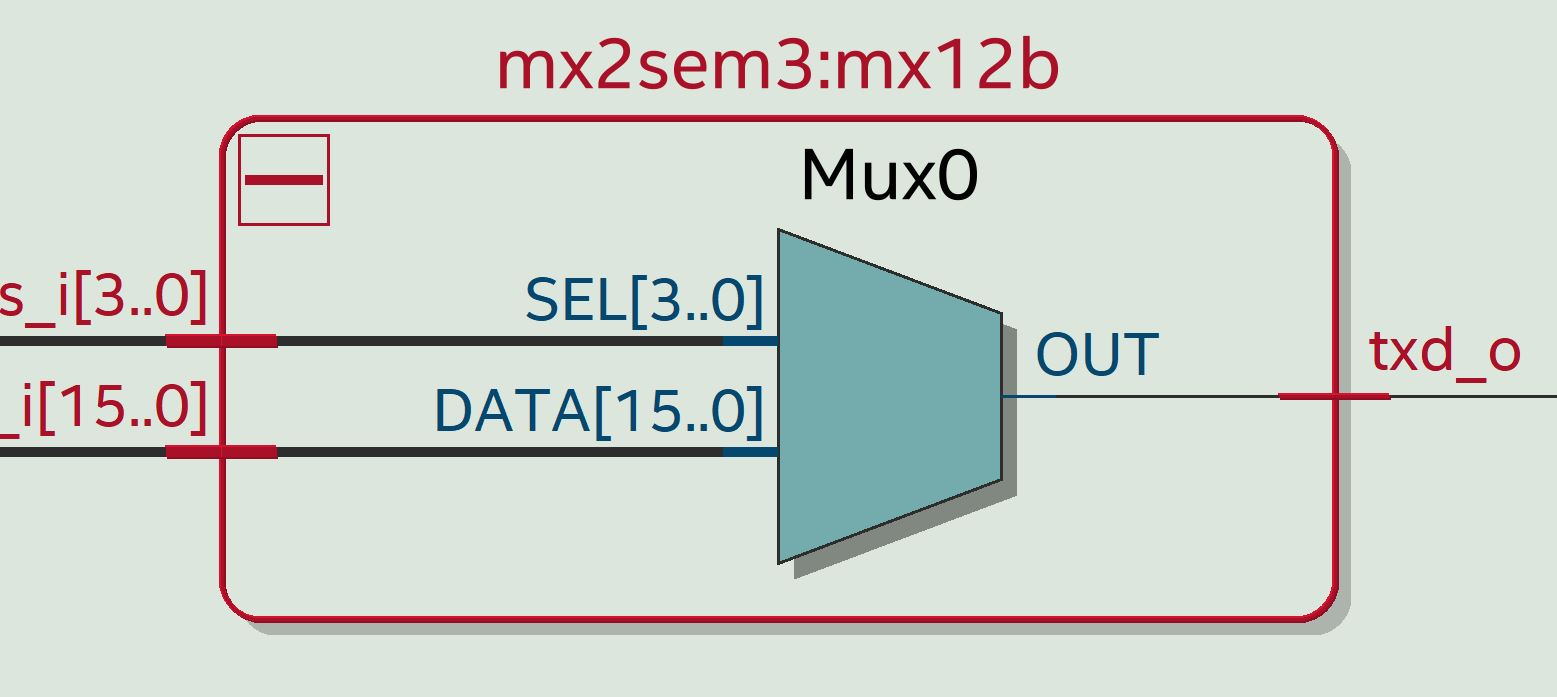
\includegraphics[width=10cm]{muxinterface.JPG}
\end{center}
Fig 11.2 S3interface multiplexer
\vspace{1 cm}
 \begin{center}
           \begin{tabular}{|c|c|c|c|}
        \hline 
        Signal  &  Full name & Type & Description \\
        \hline
        \hline
        s\_i & 4-bit selector & I &  Selector signal \\ 
        \hline
        d\_i &  16-bitdata  & I & loaded data \\
        \hline 
        txd\_o &   serial data output & O & drives S3 or µC\\
        \hline 
          \end{tabular}
\end{center}
Table 11.2 MuxInterface


\newpage
\subsection{Register}

The register is hold's the data passed in and waits till an enable signal(en\_i) is recieved. Then it passes the data out to the multiplexer.A 16-bit register is used for the S3 interface used to store the number of people(d\_s) and the event signal(event\_s) being passed.

\vspace{1 cm}
\begin{center}

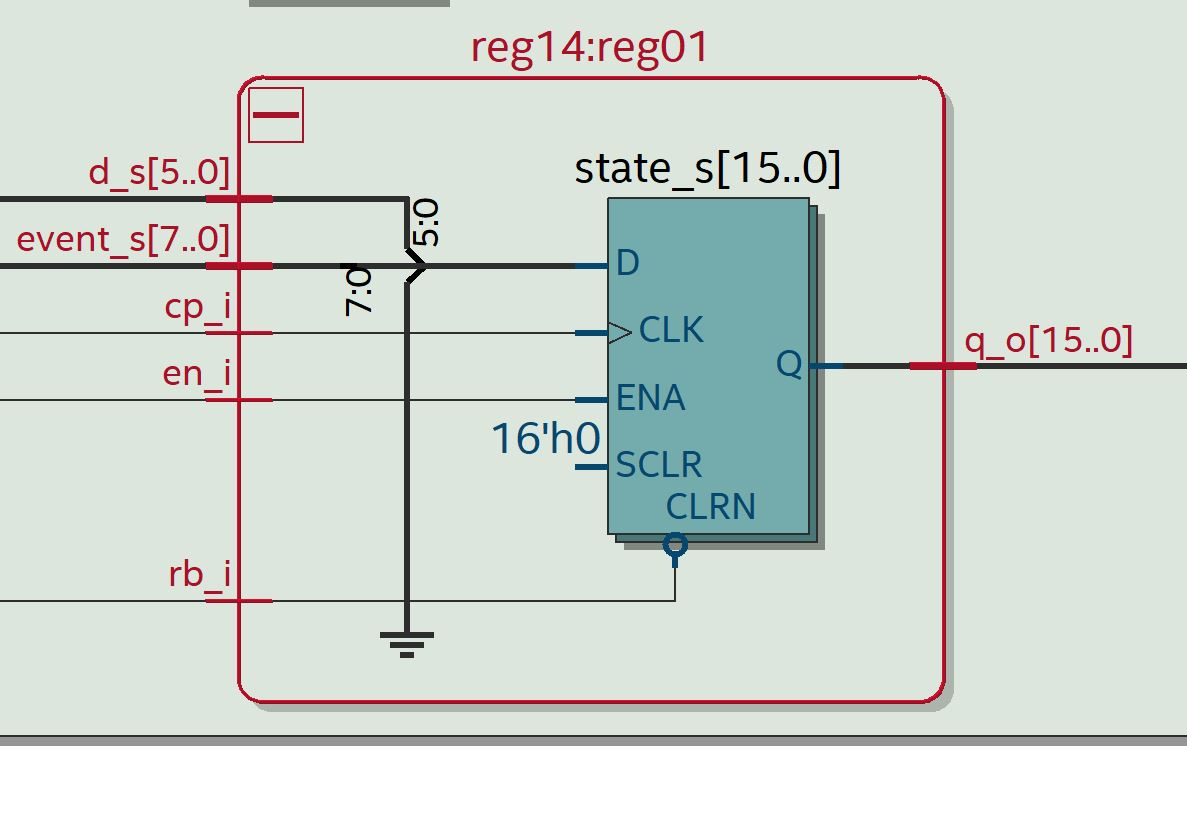
\includegraphics[width=10cm]{regs3.JPG}
\end{center}
Fig 11.3 S3interface register

\vspace{1 cm}
\begin{center}
           \begin{tabular}{|c|c|c|c|}
        \hline 
        Signal  &  Full name & Type & Description \\
        \hline
        \hline
        cp\_i & clock & I & Sys clock of 12 MHz \\
        \hline
        rb\_i & reset &  I &active low \\
        \hline
        en\_i & enable & I &start register  \\
        \hline
        d\_s & 6-bit data & I &number of people   \\ 
        \hline
        event\_s &  8-bit data  & I & +-! \\
        \hline 
        q\_o &   16-bit data & O & stored data\\
        \hline 
          \end{tabular}
\end{center}
Table 11.3 S3register

\newpage

 \section{Counter}
  
 The Baud-rate generator,UART and S3Interface consists of a counter which counts to a specific set value and when the counter reaches the specific set value sends out a pulsed signal out. The UART and The S3 interface also uses a counter but there the counter acts as a selector to select the outgoing bits from the multiplexer. For the UART and S3Interface, the counter's state changes according to an enable signal coming from the IS3 and UART FSM. 

\vspace{1.5cm}
\begin{center}

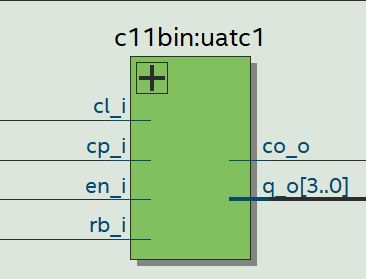
\includegraphics[width=10cm]{count.JPG}
\end{center}

Fig 12. Counter-Component

\vspace{2.5cm}
\begin{center}
           \begin{tabular}{|c|c|c|c|}
        \hline 
        Signal  &  Full name & Type & Description \\
        \hline
        \hline
        cp\_i & clock & I &Sys clock of 12 MHz \\
        \hline
        rb\_i & reset &  I & active low \\
        \hline
        en\_i & enable & I & start counter  \\
        \hline
        c\_o & carry  & O &final bit reached \\
        \hline
        q\_o &   3-bit  & O & Selector\\
        \hline 
          \end{tabular}
\end{center}

Table (I/O) Counter-Component


\section{OSI layers}
\begin{flushleft}

The OSI model \textbf{(OPEN SYSTEM INTERCONNECTION MODEL)} represents how the communication functionality of a system is working. There  are a total of  7 layers
that define the OSI model these are :  \\
\vspace{0.15cm}
\textbf{1)Physical Layer} \\
 Layer where data bits are transmitted over a physical medium\\
\vspace{0.15cm}
\textbf{2)Data link Layer}\\
Layer defines the data format\\
\vspace{0.15cm}
\textbf{3)Network Layer}  \\
Layer which defines what path the data takes\\
\vspace{0.15cm}
\textbf{4)Transport Layer} \\
Layer where the data transmission takes place with help of protocols. \\
\vspace{0.15cm}
\textbf{5)Session Layer} \\
Layer which maintains the connection between ports. \\
\vspace{0.15cm}
\textbf{6)Presentation Layer} \\
Layer which makes sure that the data is in a presentable manner, data encryption might also occurs here. \\
\vspace{0.15cm}
\textbf{7)Application Layer} \\
Layer where people can access the Network-Interface through an application \\ 
\vspace{0.5cm}
These layers can be further divided into four blocks based on their description, the Physical-Layer and the Data-Link Layer can be together  as Network-Interface-Block, Network-Layer as Internet-Block, Transport-Layer as Transport-Block and the last three layers (Session, Presentation, Application) as Application-Block.

\vspace{1cm}

\end{flushleft}
\begin{center}
           \begin{tabular}{|p{2cm}|c|p{10cm}|}
        \hline 
        Block  &  Layer & Implementation \\
        \hline
        \hline
         & Physical &  The UART-Block and the S3-Interface-Block readies raw data bits to be transmitted through  the physical communication-medium.  \\
         
        Network-Interface   & Data-Link &  The data through the UART with  1- stop- bit, packages data into groups of 8-bits, since there are no parity and check-bits there is no way to know if the data is correct.\\
        \hline
        Internet &  Network &  Since the data is transmitted through an USB cable routing is not required.\\
        \hline
        Transport & Transport &   redirecting of data is not needed \\
        \hline
                 & Session  &    Serial data communication session through the computer port and the RS232 adapter. \\
        Application   & Presentation &   Serial 8-bit data are converted  to it's corresponding decimal value  and presented in the C++ console.        \\
                    & Application  & C++ console allows the user to print out the data( number of people).           \\
        \hline
        
          \end{tabular}
\end{center}
  

\end{document}


